%%%% ijcai16.tex

\typeout{IJCAI-16 Instructions for Authors}

% These are the instructions for authors for IJCAI-16.
% They are the same as the ones for IJCAI-11 with superficical wording
%   changes only.

\documentclass{article}
% The file ijcai16.sty is the style file for IJCAI-16 (same as ijcai07.sty).
\usepackage{ijcai16}
\usepackage{algorithm}
\usepackage{algpseudocode}

\usepackage{graphicx}

\usepackage{verbatim}
\usepackage{amssymb}
\usepackage{amsmath}

\usepackage{enumitem}

\usepackage{setspace}
% Use the postscript times font!
\usepackage{times}

% the following package is optional:
%\usepackage{latexsym}


\title{Ultra-sensitive variant detection with improved accuracy using variational inference for heterogeneous next-generation sequencing data}

\author{Fan Zhang \\
Worcester Polythechnic Institute, MA  \\
fzhang@wpi.edu}

\begin{document}

\maketitle

\begin{abstract}
We propose a variational inference algorithm to estimate variant allele frequency (VAF) and identify single nucleotide variants in heterogeneous next-generation sequencing data.
We demonstrate our variational algorithm with higher sensitivity and specificity than Markov Chain Monte Carlo (MCMC) sampling method on a synthetic data set,
and more efficient at relative low median read depths of 10x and 100x.
We apply our algorithm on a longitudinal anti-cancer drug resistance sequencing data set and identify XXX variants that XXX.
We also show that our model with variational algorithm has an improved performance in XXX on a longitudinal clinical data set compared with the state of arts approaches.


\end{abstract}

\section{Introduction}
xxx\\
xxx\\
xxx\\
xxx\\
xxx\\
xxx\\
xxx\\
xxx\\
xxx\\
xxx\\
xxx\\
xxx\\
xxx\\
xxx\\
xxx\\

We show that we develop a variational expectation-maximization (EM) algorithm for our Bayesian statistical model to achieve sufficient accuracy and efficiency to identify variants in heterogeneous call samples. First, our variational EM algorithm is able to accurately approximate the posterior distribution of latent variables for a pair of samples- the sample of interest and a known reference sample. Then, a hypothesis test calls a variant by a significant difference between the key model parameters of this pair of samples. We compare the performance of variational inference algorithm to MCMC sampling method and several other variant detection methods. Finally, we demonstrate our variational algorithm on a longitudinal time-series DNA sequencing data to quantify the degree to which the variant modulates resistance to anti-cancer drug.

\section{Model Structure}
Our Bayesian statistical model is shown as a graphical representation in Figure~\ref{tbl:graphical_model}. $r_{ji}$ is the number of reads with a non-reference base at location $j$ in experimental replicate $i$. $n_{ji}$ is the total number of reads at location $j$ in experimental replicate $i$. 
\begin{figure}[htpb]
\centering
\vspace{-10pt}
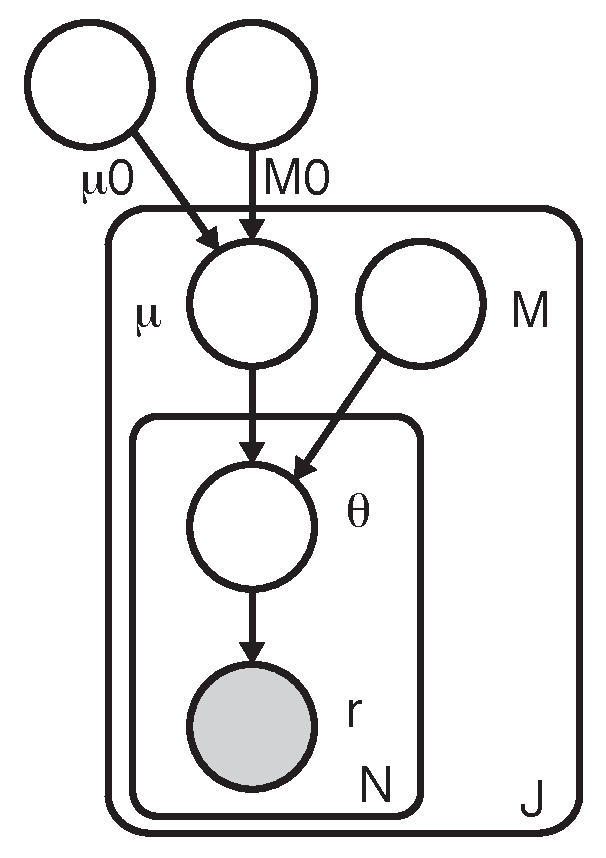
\includegraphics[width=0.18\textwidth]{figs/RVD3_model.pdf}
\caption{Graphical model representation of our Bayesian model.
$\mu_0$, a global error rate; $M_0$, a global precision;  $ \mu_j $, a local error rate. $M_j$, a local precision. $\mu_0$, a global error rate to estimate the expected error rate across all locations. $M_0$, a global precision, estimates the variation in the error rate  across locations. The local error rate, $ \mu_j $, estimates the exepected error rate across replicates at location $ j $. The local precision, $M_j$, estimates the variation in the error rate across replicates at location $j$}
\label{tbl:graphical_model}
\end{figure}
The model generative process is as follows:
\begin{enumerate}[noitemsep]
	\item For each location $j$:
	\begin{enumerate}
		\item Draw an error rate $\mu_j \thicksim \text{Beta}(\mu_0, M_0)$
		\item For each replicate $i$:
		\begin{enumerate}
			\item Draw $\theta_{ji} \thicksim \text{Beta}(\mu_j, M_j)$
			\item Draw $r_{ji} | n_{ji} \thicksim \text{Binomial}(\theta_{ji}, n_{ji})$
		\end{enumerate}
	\end{enumerate}
\end{enumerate}


\section{Inference and Hypothesis Testing}
\subsection{Variational Expectation Maximization (EM) Inference}
RVD3 improves RVD2 in the way of posterior distribution inference. We develop a non-conjugate variational inference algorithm to approximate the posterior distrubtion, 
\begin{equation}
	p(\mu, \theta | r, n; \phi)  = \frac{ p(\mu, \theta, r | n; \phi) } {p ( r | n; \phi)},
\end{equation}
where the parameters are $\phi \triangleq \{\mu_0, M_0, M\}$.
\subsubsection{Factorization}
We propose the following factorized variational distribution to approximate the true posterior over latent variables $\mu_j$ and $\theta_{ij}$. $q(\mu_j)$ approximates the variational posterior distribution of $\mu_j$, which represents the local error rate distribution in position $j$ across different replicates.
$q(\theta_{ij})$ approximates the posterior distribution of $\theta_{ij}$, which is the error rate distribution in position $j$ replicate $i$.
\begin{equation}
  q(\mu, \theta) = q(\mu)q(\theta) = \prod_{j=1}^J q(\mu_{j}) \prod_{i=1}^N q(\theta_{ji}).
  \label{eq:vardist}
\end{equation}

\subsubsection{Evidence Lower Bound (ELBO)}
The log-likelihood of the data is lower-bounded according to Jensen's inequality:
\begin{equation}
\begin{split}
\log p \left( r | \phi \right) &= \log \int_\mu \int_\theta p\left(r,\mu,\theta \right) d\theta d\mu \\
&= \log \int_\mu \int_\theta p\left(r,\mu,\theta \right)\frac{q\left(\mu,\theta \right) }{q\left(\mu,\theta \right) } d\theta d\mu \\
&\geq \int_\mu \int_\theta q\left(\mu,\theta \right) \log \frac{ p\left(r,\mu,\theta \right)}{q\left(\mu,\theta \right)} d\theta d\mu \\
&= E_q \left[ \log p\left(r,\mu,\theta \right)\right] - E_q \left[ \log q\left(\mu,\theta \right)\right] \\
&\triangleq \mathcal{L}(q, \phi).
\end{split}
\end{equation}
where $ \phi= \left( \mu_0, M_0, M \right) $.

The item $\mathcal{L}(q, \phi)$ is the evidence of lower bound (ELBO) of the log-likelihood of the data, which is the sum of $q$-expected complete log-likelihood and the entropy of the variational distribution $q$.
The goal of variational inference is maximizing the ELBO.
Equivalently, $q$ is chosen by minimizing the Kullback-Liebler (KL) divergence between the variational distribution and the true posterior distribution.

\subsubsection{Variational Distributions}
The posterior distribution of $\theta_{ij}$ is a Beta distribution,
\begin{align}
&p(\theta_{ji}|r_{ji},n_{ji},\mu_j,M_j)\\
&\thicksim \text{Beta}(r_{ji}+M_j \mu_j, n_{ji}-r_{ji}+M_j(1-\mu_j)).
\end{align}
Therefore, we propose Beta distribution with parameter vector $\delta_{ji}$ as variational distribution,
\begin{align}
\theta_{ji} &\thicksim \text{Beta}(\delta_{ji}) \nonumber
\end{align}
%
The posterior distribution of $\mu_j$ is given by its Markov blanket
\begin{align}
p(\mu_j|\theta_{ji},M_j,\mu_0,M_0)\propto p(\mu_j|\mu_0,M_0)p(\theta_{ji}|\mu_j,M_j).
\end{align}
This is not in the form of any known distribution. Therefore, we propose Beta distribution with parameter vector $\gamma_{ji}$ as variational distribution to simplify the variational derivation.
\begin{align}
\mu_j &\thicksim \text{Beta}(\gamma_j) \nonumber
\end{align}

\subsubsection{Variational Expectation Maximization (EM) Algorithm}
Variational EM maximizes the ELBO on the true likelihood, by alternating between maximization over $q$ (E-step) and maximization over $\phi$ (M-step).

\begin{algorithm}[h]
  \caption{RVD3 Variational Inference}

  \begin{algorithmic}[1]

  \State Initialize $ q(\theta, \mu) $ and $\hat{\phi}$

  \Repeat

	\Repeat
	
		\For {j = 1 to J}					
			\For {i = 1 to N}				
			\State Optimize $\mathcal{L}(q, \hat{\phi})$ over $q(\theta_{ji}; \delta_{ji}) = \text{Beta} (\delta_{ji})$				
			\EndFor			
		\EndFor
	
		\For {j = 1 to J} 		
			\State Optimize $\mathcal{L}(q, \hat{\phi})$ over $q(\mu_j; \gamma_j) = \text{Beta} (\gamma_j)$			
		\EndFor
	
	\Until{change in $\mathcal{L}(q,\hat{\phi})$ is small}

  \State Set $\hat{\phi} \leftarrow \arg \max\limits_{\phi}
            \mathcal{L}(q,\phi)$
  \Until {change in $\mathcal{L}(q,\hat{\phi})$ is small}

  \end{algorithmic}

\end{algorithm}

\section{Posterior Distribution Test}
\subsection{Z-test for Gaussian Distribution}
Variational inference provides variational distributions for $q(\mu_j|r^{control})$ and $q(\mu_j|r^{case})$, which are approximated to the posterior distributions for $p(\mu_j|r^{control})$ and $p(\mu_j|r^{case})$.
We use $Z$-test based on Gaussian distribution.
%\begin{equation}
\begin{align}
\label{eq:test}
& \mu_j^{\triangle} = \mu_j|r^{case}-\mu_j|r^{control}\\
& \sigma_j^{\triangle} = \sqrt {var_q{[\mu_j|r^{case}]} + var_q{[\mu_j|r^{control}]}}\\
& Z_j = \frac{\tau - \mu_j^{\triangle}}{{\sigma_j}^{\triangle}}\\
& Pr(Z_j) < \alpha
\end{align}
%\end{equation}
where $\tau$ is a detection threshold and $\alpha$ is a significance level. Here we set $\tau = 0$ and $\alpha = 0.05$.
$\mu_j^{case}$ and $\mu_j^{control}$ are means of distributions.
$var_q{[\mu_j|r^{case}]}$ and  $var_q{[\mu_j|r^{control}]} $are variances of distributions.
A position is called as a variant when the p-value is less than the significant level $\alpha$.

$\chi^2$ goodness-of-fit test for non-uniform base distribution is also used to distinguish a scenario of a true variant from a scenario of a random seuqencing error [cite RVD2]. 

%\subsection{Posterior Odds Ratio}

\section{Data Sets}
\subsection{Synthetic DNA Sequence Data}
xxx\\
xxx\\
xxx\\
xxx\\

\subsection{Longitudinal Drug Resistance Data}
xxx\\
xxx\\
xxx\\
xxx\\

%\subsection{Longitudinal Directed Evolution Data}

\section{Results}
\subsection{Performance on Synthetic DNA Data}

We use posterior distribution test with and without $\chi^2$ test to detect variants for a broad range of median read depths and different variant allele frequencies (VAFs).
\subsubsection{Comparison of Sensitivity and Specificity}
We compare the performance of variational algorithm and MCMC sampling method in the performance of sensitivity and specificity (Figure~\ref{tbl:statistics_mcmc_var}).
For variational algorithm, ELBO is considered as converged when the increased ELBO percent is less than $0.1\%$.
Variational algorithm with $\chi^2$ test works best compared with MCMC in sensitivity and specificity.
%The specificity is getting a little worse when the median read depth increases from $4000X$ to $400000X$ in the events of $VAF=0.1\%$, $0.3\%$, and $1.0\%$.
%The specificity is improved when tightening the stop criterion of ELBO update from $1.0\%$ to $0.1\%$.

%The specificity could be not ideal if the chosen initial values lead the variational distribution to a local optimum, which could be happened in the variational approximation algorithm. We can consider about randomly testing different initial values for $\delta$ and $\gamma$ to get rid of the local optimums results. %Threshold for $\delta$ update and $\gamma$ update is also set to guarantee its update.

% results are under folder \fzhang\Research\rvd3-variational-notebook\results\2015-09-28_Run_rvd3_synthetic_data_set
\begin{figure}[h]
\centering
\vspace{-10pt}
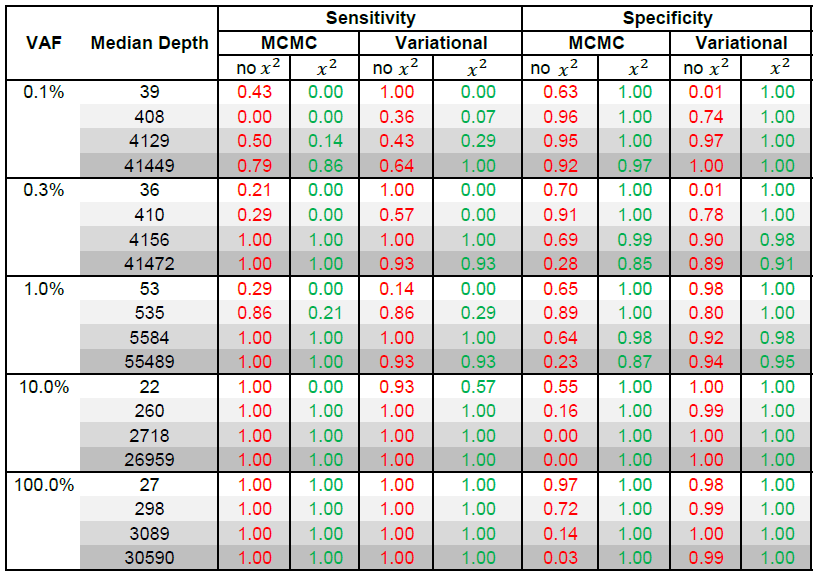
\includegraphics[width=0.5\textwidth]{figs/statistics_mcmc_var.png}
\caption{Sensitivity/Specificity comparison of variational algorithm with MCMC on the synthetic DNA data set.}
\label{tbl:statistics_mcmc_var}
\end{figure}

\subsubsection{Comparison of Approximated Posterior Distribution}
We show the approximated posterior distribution of variational algorithm and exact samples of MCMC.
A true variant position 85 of sample of VAF=$1.0\%$ is taken as an example.
Variational and MCMC both identify this position at median read depth of 5584 (Figure~\ref{tbl:posterior_mcmc_var_1}).
The specificity of variational is higher than MCMC at the highest median read depth when VAF is $0.1\%$, $0.3\%$, and $1.0\%$ , which shows that MCMC calls more false positive positions.
Here we show the approximated distribution of a false positive position 144 identified by MCMC, while it is not identified by variational algorithm (Figure~\ref{tbl:posterior_mcmc_var_3}).
It is noticeable that the shape of variational distributions using Beta distribution is very close to Gaussian distribution.

% results are under folder \fzhang\Research\rvd3-variational-notebook\results\2015-10-14_Plot_mcmc_mu_vs_variational_mu
\begin{figure}[h]
\centering
\vspace{-10pt}
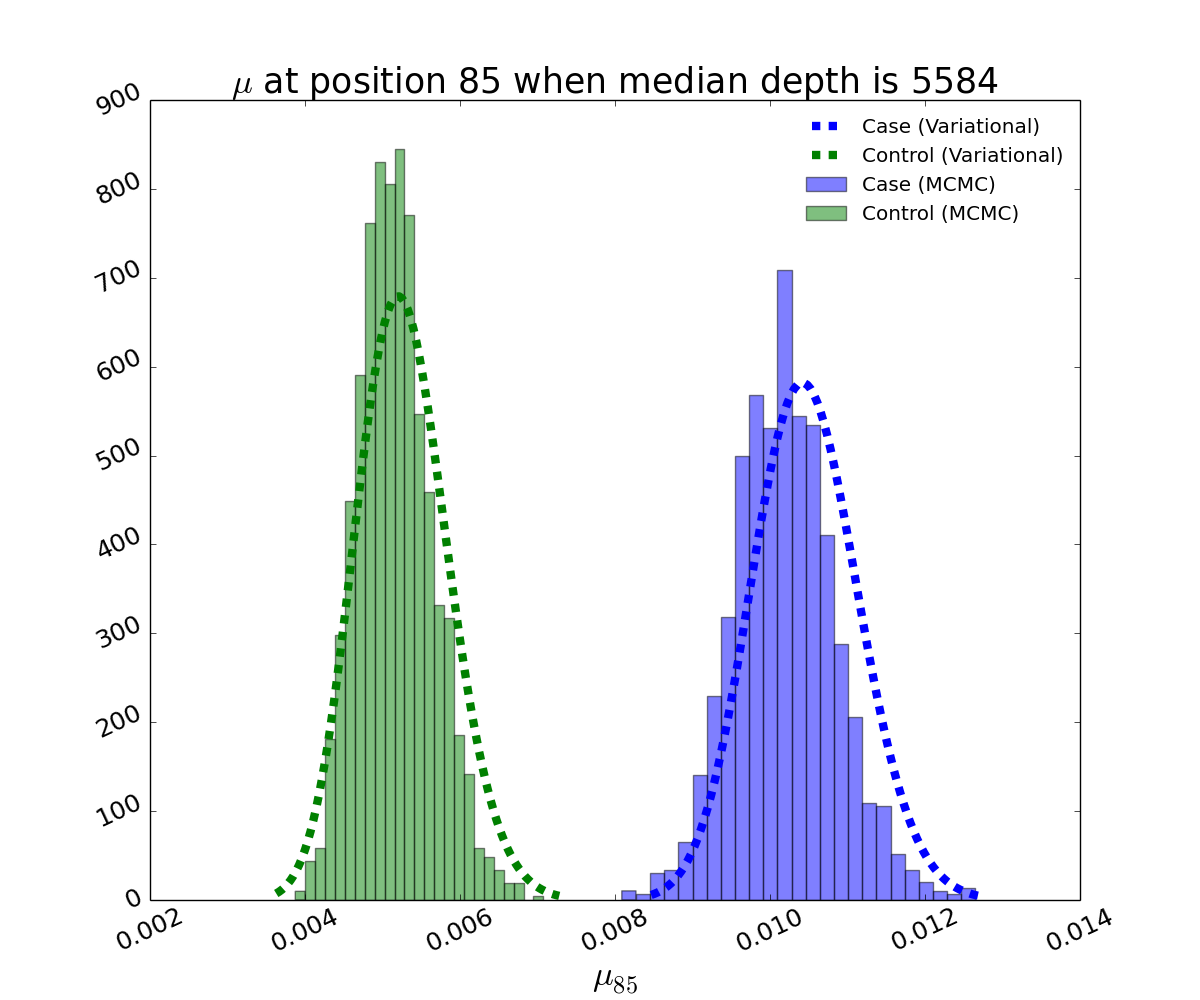
\includegraphics[width=0.4\textwidth]{figs/position_85_5584_mcmc_vs_var_mu.png}
\caption{Approximated posterior distribution by variational algorithm and MCMC for position 85 when median read depth is 5584.}
\vspace{-10pt}
\label{tbl:posterior_mcmc_var_1}
\end{figure}

%\begin{figure}[h]
%\centering
%\vspace{-10pt}
%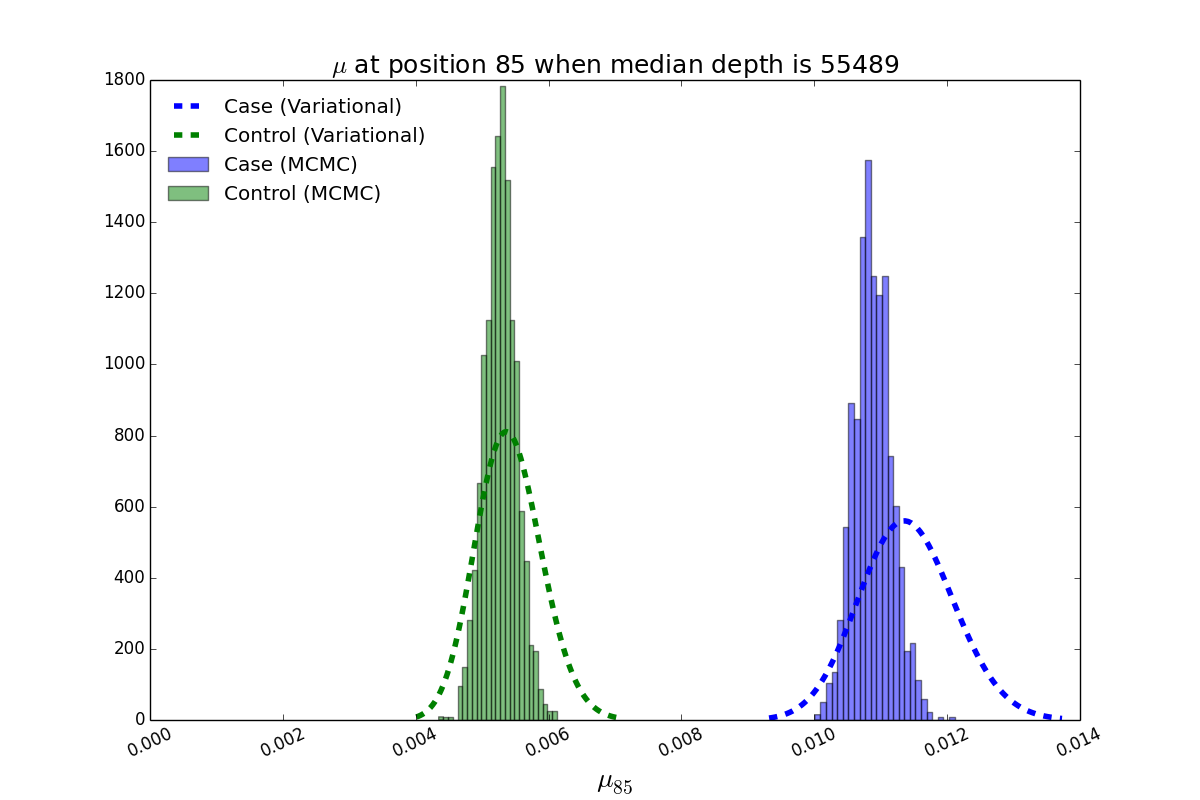
\includegraphics[width=0.5\textwidth]{figs/position_85_55489_mcmc_vs_var_mu.png}
%\caption{Approximated posterior distribution by variational algorithm and MCMC for position 85 when median read depth is 55489.}
%\vspace{-10pt}
%\label{tbl:posterior_mcmc_var_2}
%\end{figure}

\begin{figure}[!htbp]
\centering
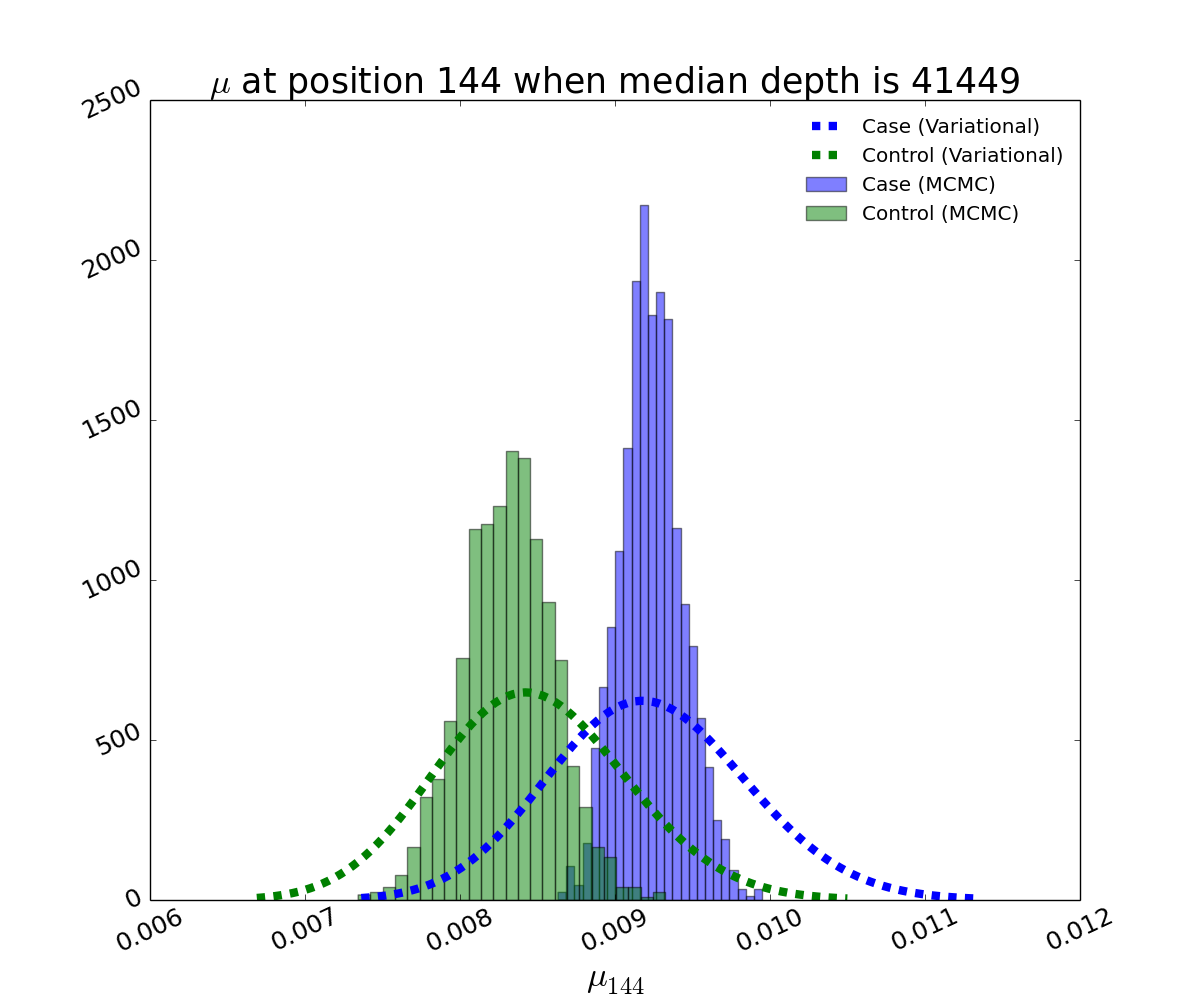
\includegraphics[width=0.4\textwidth]{figs/position_144_41449_mcmc_vs_var_mu.png}
\caption{Approximated posterior distribution of position 144 when median read depth is 41449. This is a false positive position identified by MCMC, while variational algorithm does not identify this as a variant.}
\vspace{-10pt}
\label{tbl:posterior_mcmc_var_3}
\end{figure}

\subsubsection*{Comparison of Timing}
Time for approximating variational posterior distribution is increased by increasing the length of region of interest and the median read depth (Figure~\ref{tbl:timing_mcmc_var}).
Variational algorithm works faster than MCMC at low read depths (27x and 298x), while MCMC works faster than variational algorithm at high read depths (3089x and 30590x).

% results are under folder \fzhang\Research\rvd3-variational-notebook\results\2015-10-15_Plot_time_vs_region_length_rvd3_synthetic_data
\begin{figure}[htbp]
\centering
\vspace{-10pt}
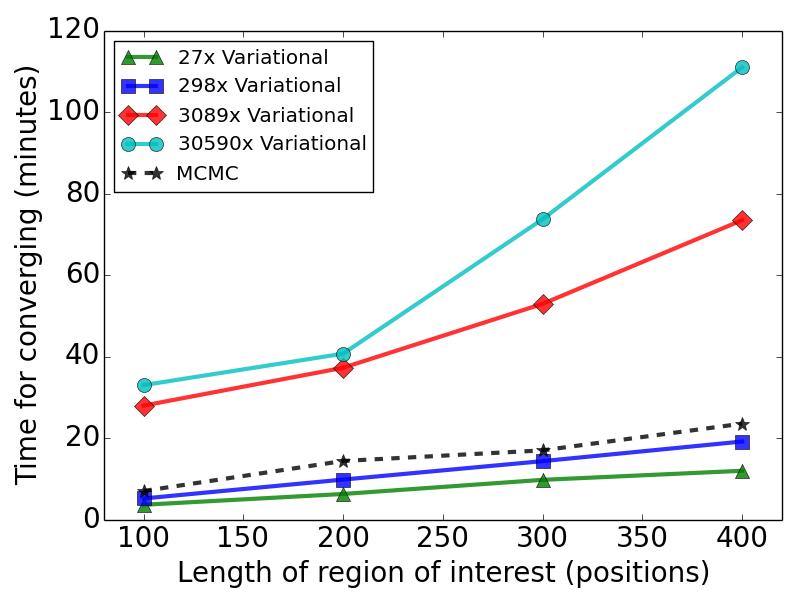
\includegraphics[width=0.5\textwidth]{tables/timing_var_mcmc.png}
\caption{Timing figure for variational algorithm and MCMC method.
60 processes are used to estimate the model on the synthetic data set.}
\vspace{-10pt}
\label{tbl:timing_mcmc_var}
\end{figure}

Timing profile for each parts of variational algorithm is also given in Figure~\ref{tbl:timing_profile_all}.
Optimizing $\gamma$ function in E-step and optimizing $M$ in M-step takes most of the time because an integration is needed.

% results are under folder \fzhang\Research\rvd3-variational-notebook\results\2015-10-21_Timing_profile_rvd3_program
\begin{figure*}{b}
\centering
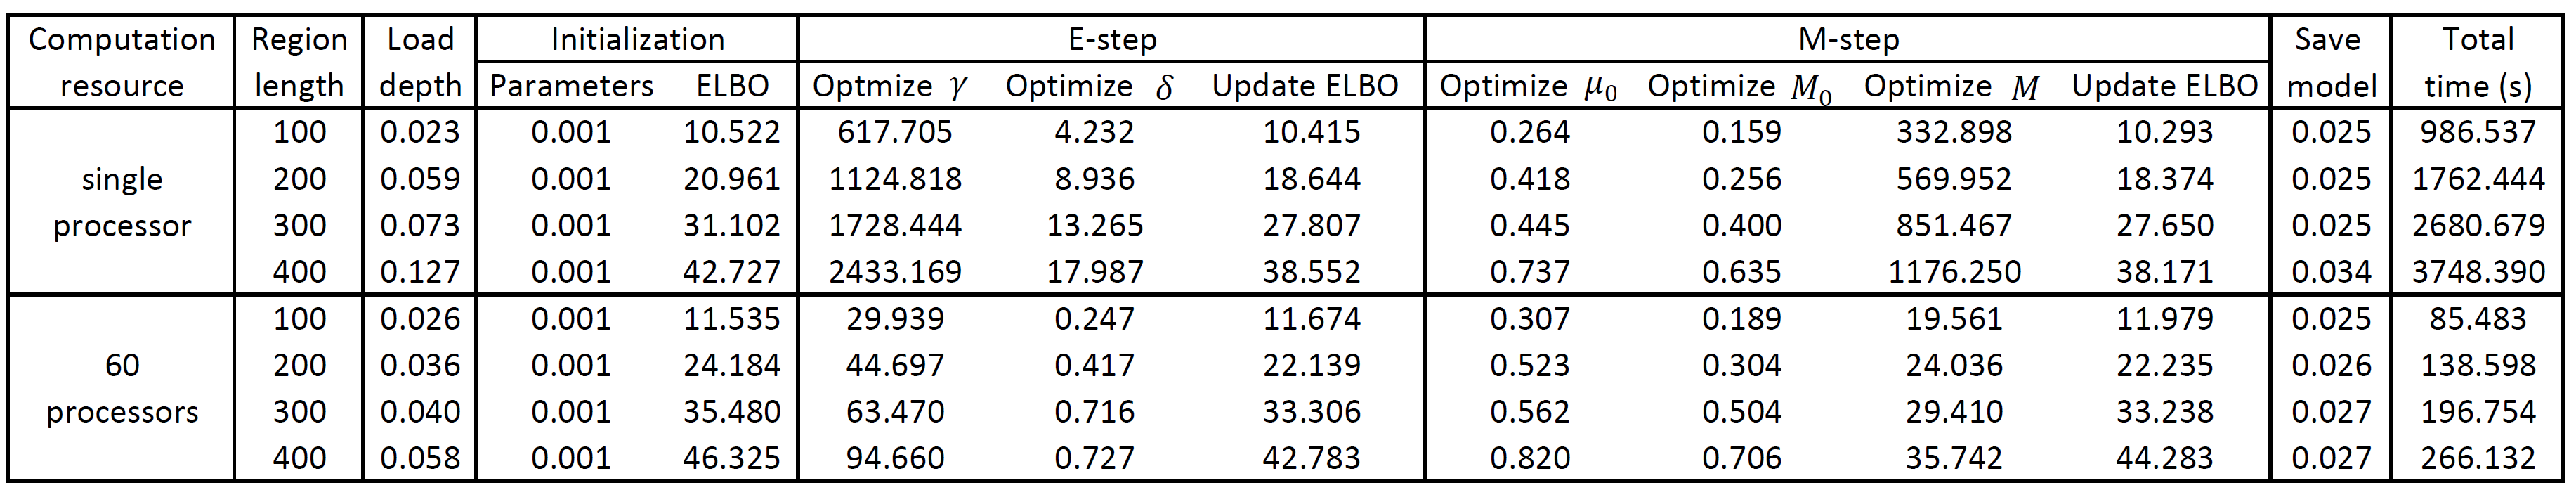
\includegraphics[width=1.0\textwidth]{tables/time_3089X_all.png}
\caption{Timing profile for one iteration of variational EM algorithm.
Single and multiple processors are both tested for timing to estimate the model on the synthetic data set.}
\vspace{-10pt}
\label{tbl:timing_profile_all}
\end{figure*}

\subsection{Variants Detection on the Longitudinal Drug Resistance Data}
\subsubsection{Detected Drug Resistance Variants}
xxx\\
xxx\\
xxx\\
xxx\\
xxx\\
xxx\\
xxx\\
xxx\\
xxx\\
xxx\\
xxx\\
xxx\\
xxx\\
xxx\\
xxx\\

\subsubsection{Comparison to the State of Arts Approaches}
xxx\\
xxx\\
xxx\\
xxx\\
xxx\\
xxx\\
xxx\\
xxx\\
xxx\\
xxx\\
xxx\\
xxx\\
xxx\\
xxx\\

\subsection{Discussion}
xxx\\
xxx\\
xxx\\
xxx\\
xxx\\
xxx\\
xxx\\
xxx\\
xxx\\
xxx\\
xxx\\
xxx\\
xxx\\
xxx\\
xxx\\
xxx\\
xxx\\

\section*{Acknowledgments}
Funding:


\appendix
%\section{Derivation of Variational Inference}

%% The file named.bst is a bibliography style file for BibTeX 0.99c
\bibliographystyle{named}
\bibliography{ijcai16}

\end{document}

